% Resultados da aplicação (trilha EC): previsão do atraso crítico e montagem HIL no Tinkercad

\textbf{Previsão pelo critério de Nyquist.} Sem atraso, o laço PID do Sistema D tem MF de \MFsemAtraso$^\circ$ em $\omega_{cg}=\WcgD$~rad/s. Logo, o critério prevê instabilidade para um atraso total acima de $\tau_{crit}=\TauCrit$~s, valor confirmado por bissecção sobre o veredito $Z$ do próprio Nyquist (\TauCritBis~s).

\textbf{Gêmeo digital.} A Tabela~\ref{tab:hil-ts} compara a previsão contínua com o menor atraso, em amostras, que torna instável o laço discreto simulado pelo gêmeo, avaliado pela taxa de crescimento da envoltória do erro, sem saturação. Com $T_s=5$~ms, o limite discreto (\TauHilFino~s) praticamente coincide com a previsão corrigida pelo atraso equivalente do ZOH ($\tau_{crit}-T_s/2$). Para períodos maiores, a instabilidade surge cerca de uma amostra antes do previsto, o que é coerente com o atraso de fase adicional da discretização do PID (Euler para trás). Com o período adotado nos \textit{sketches} ($T_s=20$~ms), o limite previsto é de \DcritHil\ amostras (\TauHil~s).

\begin{table}[ht]
\centering
\caption{Atraso crítico: previsão de Nyquist (tempo contínuo) e laço discreto do gêmeo digital.}
\label{tab:hil-ts}
\small
\resizebox{\textwidth}{!}{\begin{tabular}{lccccc}
\hline
$T_s$ (ms) & $d_{crit}$ (amostras) & $\tau$ simulado (s) & $\tau$ Nyquist (s) & $\tau$ Nyquist $- T_s/2$ (s) & Desvio (\%) \\
\hline
5 & 224 & 1{,}120 & 1{,}122 & 1{,}119 & -0{,}18 \\
10 & 111 & 1{,}110 & 1{,}122 & 1{,}117 & -1{,}07 \\
20 & 55 & 1{,}100 & 1{,}122 & 1{,}112 & -1{,}96 \\
50 & 22 & 1{,}100 & 1{,}122 & 1{,}097 & -1{,}96 \\
\hline
\end{tabular}
}
\end{table}

\textbf{Simulação no Tinkercad.} A Figura~\ref{fig:tinkercad-circuito} mostra o circuito montado no Tinkercad Circuits, com os dois Arduinos ligados em cruz pela serial (TX$\to$RX), o potenciômetro que ajusta o atraso, a chave de atraso variável e o LED ``L'' da Planta, que acende quando $|r-y|>0{,}5$ após 10~s. Os ensaios foram executados pelo próprio simulador, e a série completa $y[k]$, $\tau[k]$, $u[k]$ de cada ensaio foi capturada do Monitor Serial da Planta. A Figura~\ref{fig:tinkercad-monitor} mostra a tela do simulador durante o ensaio acima do limite.

\begin{figure}[ht]
\centering
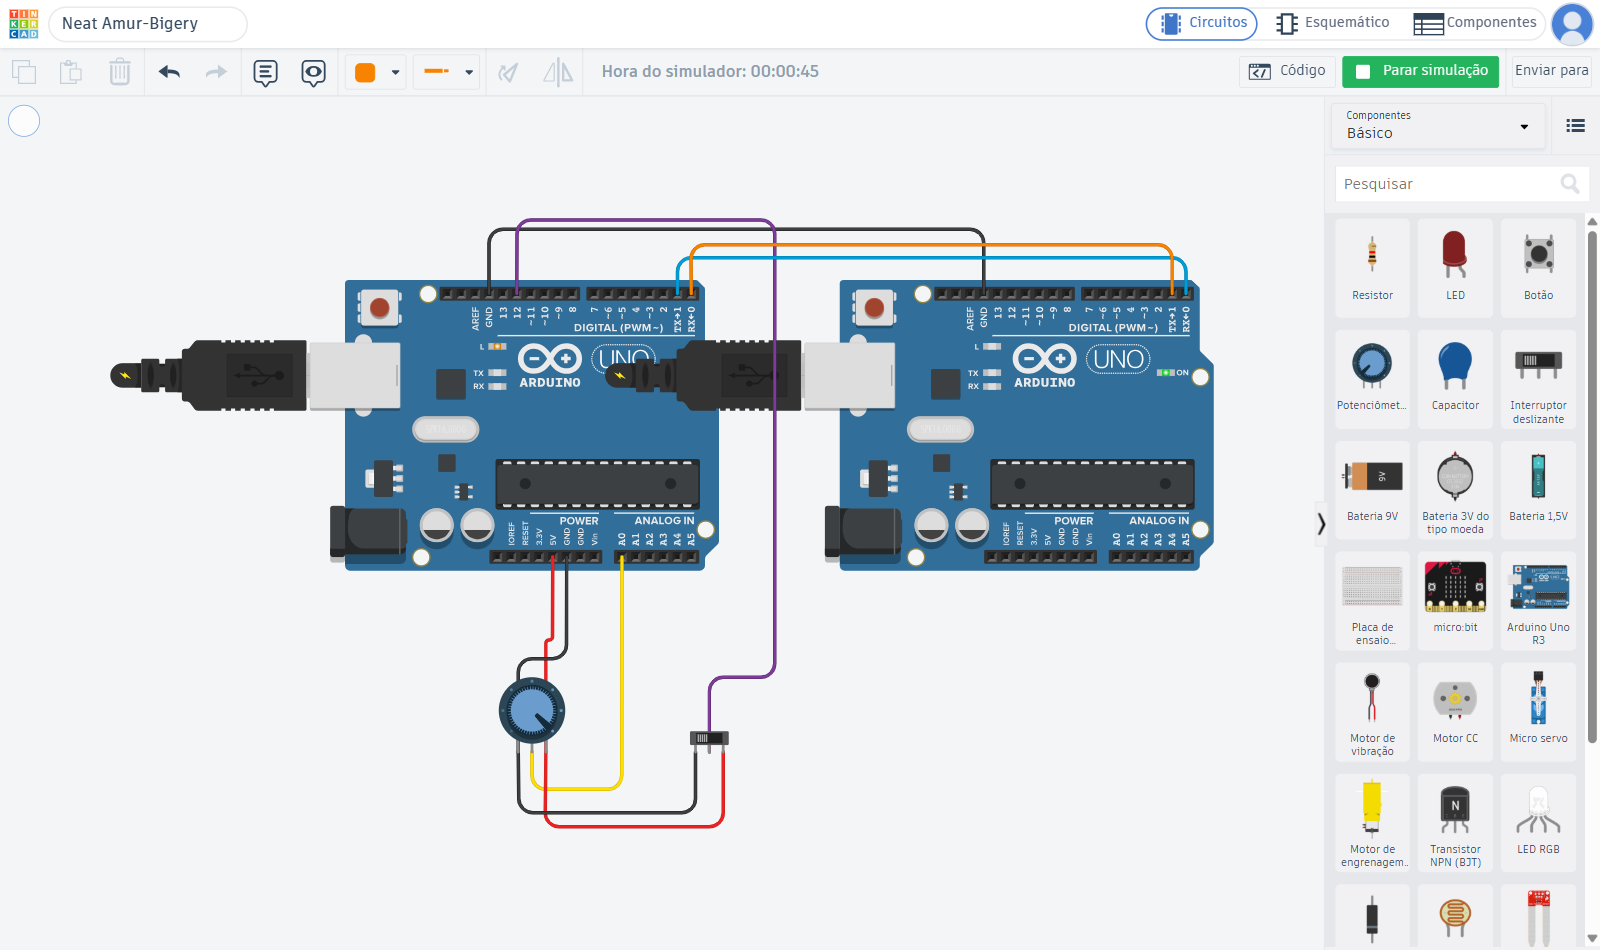
\includegraphics[width=\textwidth,trim=90 110 380 200,clip]{T5_circuito_0.png}
\caption{Circuito HIL simulado no Tinkercad: Arduino ``Planta'' (esquerda) e Arduino ``Controlador'' (direita). Captura feita durante o ensaio T5 ($\tau=1{,}20$~s), com o LED ``L'' da Planta aceso pela oscilação crescente.}
\label{fig:tinkercad-circuito}
\end{figure}

\begin{figure}[ht]
\centering
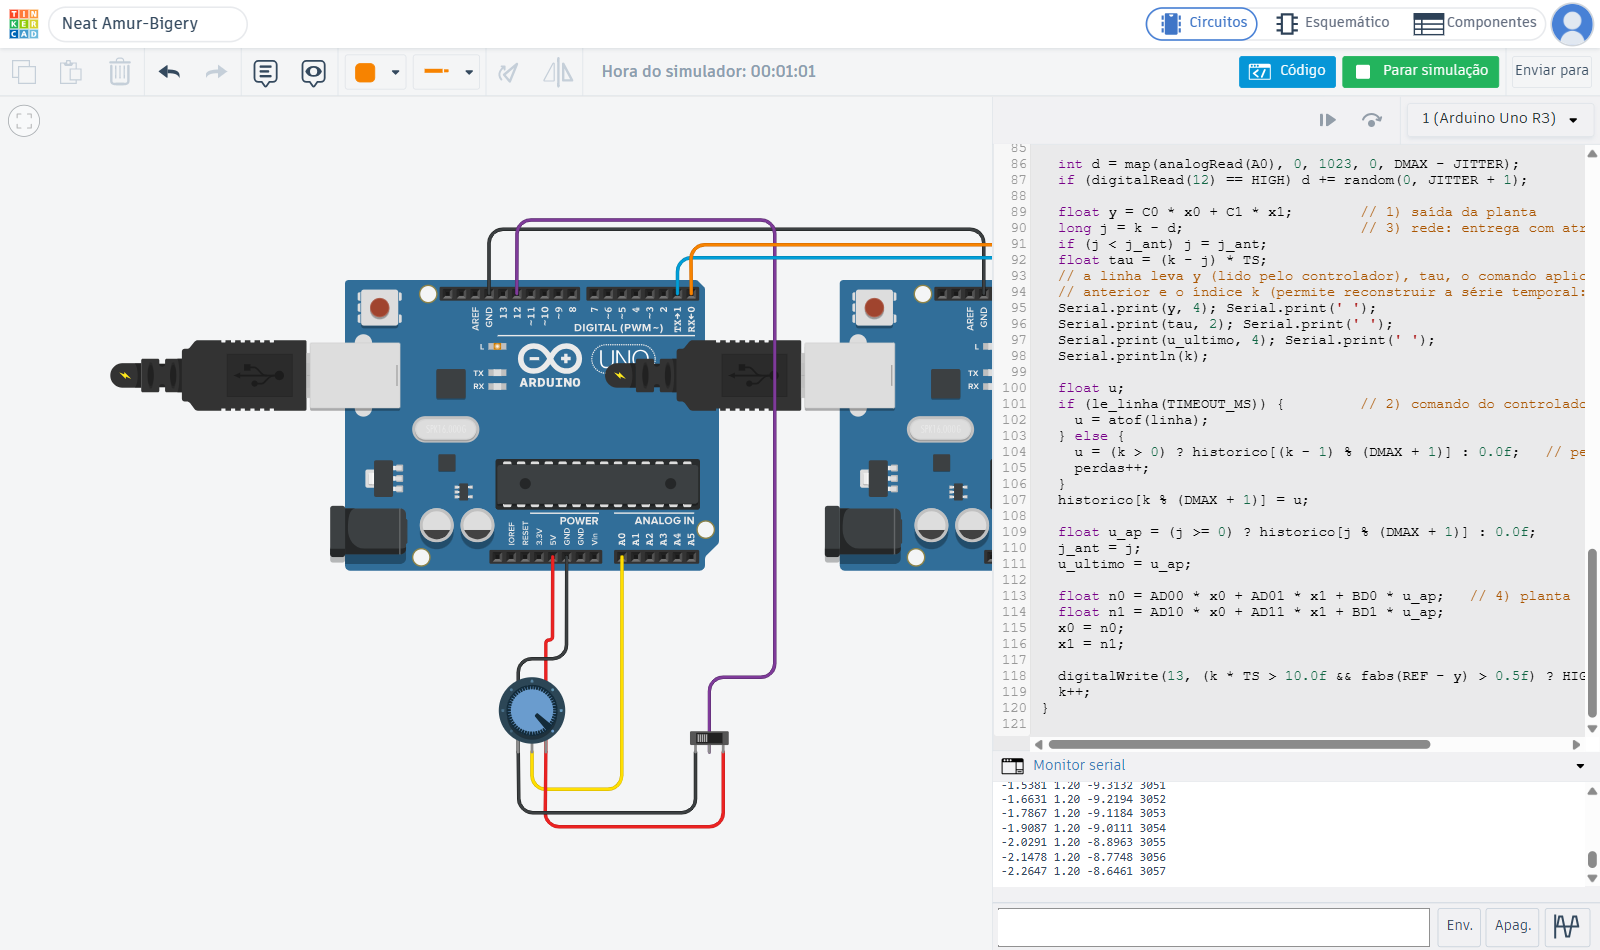
\includegraphics[width=\textwidth]{T5.png}
\caption{Tela do Tinkercad durante o ensaio T5: código da Planta e Monitor Serial com as colunas $y$, $\tau$, $u$ e $k$. O relógio do simulador indica o tempo simulado.}
\label{fig:tinkercad-monitor}
\end{figure}

A Tabela~\ref{tab:tinkercad} e a Figura~\ref{fig:tinkercad-resp} resumem os ensaios. Nos ensaios com atraso fixo, o traço do Tinkercad coincide com o do gêmeo digital, amostra a amostra, com erro máximo de $\ErroTinkMax$, limitado pelas quatro casas decimais da impressão serial. Isso mostra que o comportamento observado no simulador é o do algoritmo especificado, e não um efeito do ambiente. O limite de estabilidade medido no Tinkercad ficou entre $d=\TkQuatroaD$ amostras, que decai com taxa $\TkQuatroaTaxa$~s$^{-1}$, e $d=\TkQuatrobD$ amostras, que cresce com taxa $+\TkQuatrobTaxa$~s$^{-1}$. Esse limite coincide com o do gêmeo e fica a menos de uma amostra (2\%) da previsão do critério de Nyquist em tempo contínuo. O ensaio T5 ($\tau=1{,}20$~s) mostra a oscilação crescente que, com a saturação do atuador, evolui para um ciclo-limite de grande amplitude.

\begin{table}[ht]
\centering
\caption{Ensaios executados no Tinkercad (taxa: crescimento exponencial da envoltória do erro; negativa = estável).}
\label{tab:tinkercad}
\small
\begin{tabular}{lccccc}
\hline
Ensaio & $\tau$ (s) & Pico de $y$ & Taxa (1/s) & Veredito & Erro máx. x gêmeo \\
\hline
T1 & 0{,}00 & 1{,}000 & -- & estável & $9{,}3 \times 10^{-5}$ \\
T2 & 0{,}50 & 1{,}240 & -- & estável & $7{,}4 \times 10^{-5}$ \\
T3 & 1{,}00 & 1{,}822 & -0{,}0467 & estável & $7{,}8 \times 10^{-5}$ \\
T4a & 1{,}08 & 1{,}913 & -0{,}0077 & estável & $8{,}7 \times 10^{-5}$ \\
T4b & 1{,}10 & 2{,}050 & 0{,}0009 & instável & $1{,}2 \times 10^{-4}$ \\
T4c & 1{,}12 & 2{,}687 & 0{,}0091 & instável & $8{,}7 \times 10^{-5}$ \\
T5 & 1{,}20 & 5{,}555 & 0{,}0382 & instável & $1{,}3 \times 10^{-4}$ \\
T6 & 0{,}80--1{,}12 & 1{,}738 & -0{,}1507 & estável & $2{,}3 \times 10^{-4}$ \\
\hline
\end{tabular}

\end{table}

\begin{figure}[ht]
\centering
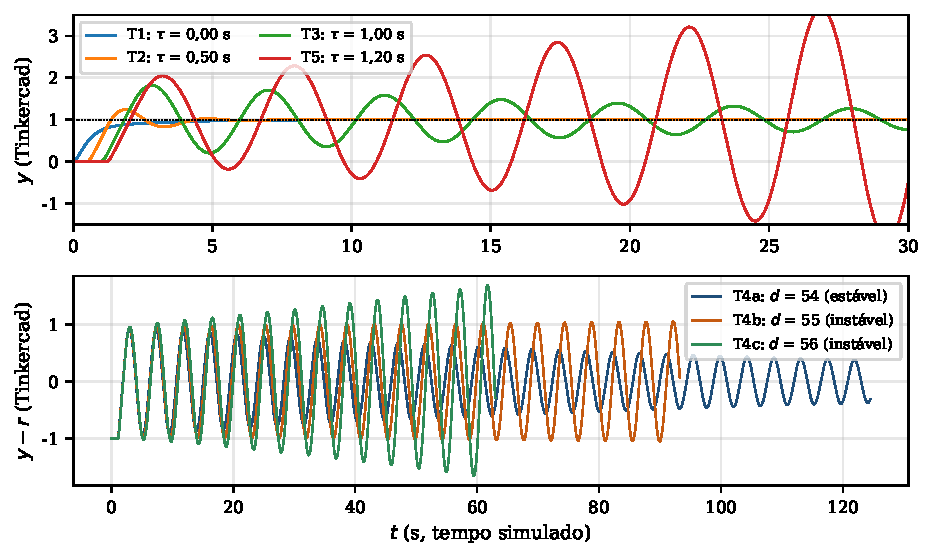
\includegraphics[width=\textwidth]{tinkercad_respostas.pdf}
\caption{Respostas ao degrau medidas no Tinkercad. Acima: ensaios com atraso fixo. Abaixo: erro em torno do limite de estabilidade ($d=54$, $55$ e $56$ amostras).}
\label{fig:tinkercad-resp}
\end{figure}

\textbf{Atraso variável.} No ensaio T6, a chave ativa um atraso sorteado a cada período em $[d,d+20]$ amostras, com base em $d=40$ ($0{,}80$~s). Como os pacotes são entregues em ordem, um pacote não pode ser aplicado antes de um mais antigo. Por isso, o atraso efetivo cresce uma amostra por período até que um sorteio menor libere um pacote mais recente, e permanece próximo do limite inferior da faixa. A estabilidade é, então, governada pelo atraso \emph{mínimo}, e não pelo médio. O gêmeo digital reproduz esse comportamento: com sorteios em $[56,76]$, a malha é instável, enquanto com $[50,70]$ ainda é estável, embora o atraso médio desta última faixa supere o limite para atraso constante. Reproduzindo no gêmeo a mesma sequência de atrasos efetivos registrada no Tinkercad, o erro máximo entre os traços do ensaio T6 foi de $\TkSeisErro$.
